
\documentclass{article}
\usepackage{lmodern}
\usepackage[T1]{fontenc}
\usepackage{shapepar}
\usepackage{microtype}
\usepackage{lipsum}
\usepackage{pgfplots}
\pgfplotsset{compat=1.9}
\usepackage{tikz}
\usetikzlibrary{calc,fit,intersections,folding}
\usepackage{pstricks-add}
\usetikzlibrary{arrows.meta,angles,arrows,quotes,backgrounds,calc}
\usepackage[left = 5mm, right = 5mm, top = 5mm, bottom = 5mm]{geometry}



\setlength{\parindent}{0em}

\newcommand{\clrone}{blue}
\newcommand{\clrtwo}{red}

\begin{document}
\thispagestyle{empty}

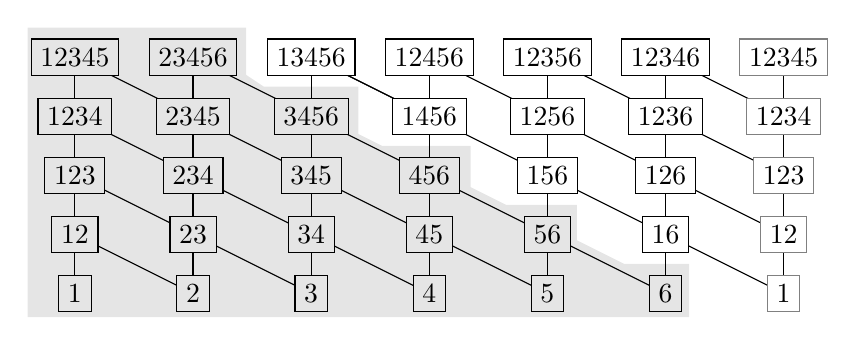
\begin{tikzpicture}[scale = 1.5,yscale = 0.5]

\coordinate (1) at (0,0);
\coordinate (2) at (1,0);
\coordinate (3) at (2,0);
\coordinate (4) at (3,0);
\coordinate (5) at (4,0);
\coordinate (6) at (5,0);
\coordinate (1e) at (6,0);

\coordinate (12) at (0,1);
\coordinate (23) at (1,1);
\coordinate (34) at (2,1);
\coordinate (45) at (3,1);
\coordinate (56) at (4,1);
\coordinate (16) at (5,1);
\coordinate (12e) at (6,1);

\coordinate (123) at (0,2);
\coordinate (234) at (1,2);
\coordinate (345) at (2,2);
\coordinate (456) at (3,2);
\coordinate (156) at (4,2);
\coordinate (126) at (5,2);
\coordinate (123e) at (6,2);

\coordinate (1234) at (0,3);
\coordinate (2345) at (1,3);
\coordinate (3456) at (2,3);
\coordinate (1456) at (3,3);
\coordinate (1256) at (4,3);
\coordinate (1236) at (5,3);
\coordinate (1234e) at (6,3);

\coordinate (12345) at (0,4);
\coordinate (23456) at (1,4);
\coordinate (13456) at (2,4);
\coordinate (12456) at (3,4);
\coordinate (12356) at (4,4);
\coordinate (12346) at (5,4);
\coordinate (12345e) at (6,4);

\foreach \a/\b in {1/12,12/123,123/1234,1234/12345,2/12,2/23,23/123,23/234,234/1234,234/2345,2345/12345,2345/23456,3/23,3/34,34/234,34/345,345/2345,345/3456, 3456/23456,3456/13456, 4/34,4/45,45/345,45/456, 456/3456,456/1456,1456/13456,1456/12456, 5/45,5/56,56/456,56/156,156/1456,1456/13456,1456/12456, 156/1256,1256/12456,1256/12356,6/56,6/16,16/156/16/126,126/1256,126/1236,1236/12356,1236/12346,16/126, 1e/16,1e/12e,12e/126,12e/123e,123e/1236,123e/1234e,1234e/12346,1234e/12345e}
{\draw (\a) -- (\b);}

\foreach\n in {1,2,3,4,5,6,12,23,34,45,56,16,123,234,345,456,156,126,1234,2345,3456,1456,1256,1236,12345,23456,13456,12456,12356,12346}
{\node[draw, fill=white] at (\n) {$\n$}; }

\node[draw = gray, fill=white] at (1e) {$1$};
\node[draw = gray, fill=white] at (12e) {$12$};
\node[draw = gray, fill=white] at (123e) {$123$};
\node[draw = gray, fill=white] at (1234e) {$1234$};
\node[draw = gray, fill=white] at (12345e) {$12345$};

\fill[opacity = 0.1] (-0.4,4.5) -- (1.45,4.5) -- (1.45,3.7) -- (1.6,3.5) -- (2.4,3.5) -- (2.4,2.7) -- (2.6,2.5) -- (3.35,2.5) -- (3.35,1.8) -- (3.65,1.5) -- (4.25,1.5) -- (4.25,0.9) -- (4.65,0.5) -- (5.2,0.5) -- (5.2,-0.4) -- (-0.4,-0.4) -- cycle;

\end{tikzpicture}

\end{document}
